\section{CÁC PHÉP TOÁN TRÊN TẬP HỢP}

\subsection{TÓM TẮT LÝ THUYẾT}
\subsubsection{Hợp của hai tập hợp}
\immini{\begin{itemize}
		\item  $A\cup B=\{x|x\in A$ hoặc $x\in B \} $.
		\item  Ghi nhớ: Lấy hết phần tử của cả hai tập, các phần tử trùng nhau thì ta ghi 1 lần.
\end{itemize}}{
	\begin{tikzpicture}[smooth,font=\footnotesize,scale=0.8]
		\draw[pattern=north east lines,pattern color=orange]
		(0,0) to[bend left=90] (2,2) to[bend left=90] (0,0)
		(1,0) to[bend left=90] (3,2) to[bend left=90] (1,0)
		(1,-0.7) node{Biểu đồ Venn minh họa $A \cup B$}
		(0.5,1) node{$A$}
		(2.6,0.9) node{$B$};
\end{tikzpicture}}

\subsubsection{Giao của hai tập hợp}
\immini{\begin{itemize}
		\item  $A\cap B= \{x|x\in A$ và $x\in B \}$.
		\item  Ghi nhớ: Lấy phần chung của 2 tập hợp.
\end{itemize}}{
	\begin{tikzpicture}[smooth,font=\footnotesize,scale=0.8]
		\def\miena{(0,0) to[bend left=90] (2,2) to[bend left=90] (0,0)}
		\def\mienb{(1,0) to[bend left=90] (3,2) to[bend left=90] (1,0)}
		\begin{scope}
			\clip \miena;
			\draw[pattern=north east lines,pattern color=orange] \mienb;
		\end{scope}
		\draw \miena \mienb
		(1,-0.7) node{Biểu đồ Venn minh họa $A \cap B$}
		(0.5,1) node{$A$}
		(2.6,0.9) node{$B$};
\end{tikzpicture}}
\subsubsection{Hiệu của hai tập hợp, phần bù của tập con}
\begin{itemize}
		\item  $A\backslash B= \{x|x\in A$ và $x\notin B \} $.
		\item  Ghi nhớ: Lấy phần riêng (thuộc A mà không thuộc B).
		\item Đặc biệt: Nếu $B\subset A$ thì $A\backslash B$ được kí hiệu là \fbox{$C_AB$} (gọi là phần bù của $B$ trong $A$).
\end{itemize}
\hspace*{2cm}
\begin{tikzpicture}[smooth,font=\footnotesize,scale=1]
	\def\miena{(0,0) to[bend left=90] (2,2) to[bend left=90] (0,0)}
	\def\mienb{(1,0) to[bend left=90] (3,2) to[bend left=90] (1,0)}
	\fill[pattern=north east lines,pattern color=orange] \miena;
	\draw[fill=white] \mienb
	(1,-0.7) node{Biểu đồ Venn minh họa $A \backslash B$}
	(0.5,1) node{$A$}
	(2.6,0.9) node{$B$};
	\draw \miena ;
\end{tikzpicture}
\hspace{3cm}
\begin{tikzpicture}[smooth,font=\footnotesize,scale=1]
	\def\miena{(0,0) to[bend left=90] (2,2) to[bend left=90] (0,0)}
	\def\mienb{(0.5,0.5) to[bend left=90] (1.5,1.75) to[bend left=90] (0.5,0.5)}
	\draw[pattern=dots,pattern color=orange] \miena;
	\draw[fill=white] \mienb
	(1,-0.7) node{Biểu đồ Venn minh họa phần bù của $B$ trong $A$}
	(1,1.2) node{$B$}
	(0.5,0.1) node{$C_AB$}
	(2.3,0.8) node{$A$};
	\end{tikzpicture}
\subsection{RÈN LUYỆN KĨ NĂNG GIẢI TOÁN}

\begin{dang}{Các phép toán trên tập hợp}
\end{dang}

\begin{vd}
	Cho hai tập hợp $A=\left\{0;1;2;3;4\right\}$ và $B=\left\{2;3;4;5;6\right\}$. Tìm các tập hợp $A\cup B, A\cap B, A\backslash B, B\backslash A$.
	\loigiai{
		Ta có $A\backslash B=\left\{0;1\right\}$, $B\backslash A=\left\{5;6\right\}$, $A\cup B=\left\{0;1;2;3;4;5;6\right\}$, $A\cap B=\left\{2;3;4\right\}$.
	}
\end{vd}\dongcham{4}



\begin{vd}
	Cho $A=\left\{x\in \left. \mathbb{N}\right|\right.x\le \left. 5\right\}$, $B=\left\{x\in \left. \mathbb{N}\right|\right.x=3k-1,k\in \mathbb{N},k\le \left. 3\right\}$. Xác định tập $A, B, A\cap B, A\cup B, A\backslash B, B\backslash A$.
	\loigiai{
		Ta có $A=\left\{0;1;2;3;4;5\right\}$ và $B=\left\{-1;2;5;8\right\}$ nên
		\begin{enumEX}[+]{2}
			\item $A\cap B=\left\{2;5\right\}$,
			\item $A\cup B=\left\{-1;0;1;2;3;4;5;8\right\}$,
			\item $A\backslash B=\left\{0;1;3;4\right\}$,
			\item $B\backslash A=\left\{-1;8\right\}$.
		\end{enumEX}
	}
\end{vd}\dongcham{6}

\begin{vd}
	Cho tập hợp $E=\left\{1;2;3;4;5;6;7;8;9\right\}$ và các tập hợp con $A=\left\{1;2;3;4\right\}$, $B=\left\{2;4;6;8\right\}$. Xác định $C_EA$, $C_EB$, $C_E\left(A\cup B\right)$, $C_EA\cap C_EB$.
	\loigiai{\\
		Ta có 
		\begin{enumerate}[$\bullet$]
			\item $C_EA=E\backslash A=\left\{5;6;7;8;9\right\}$
			\item $C_EB=E\backslash B=\left\{1;3;5;7;9\right\}$ 
			\item  $C_EA\cap C_EB=\left\{5;7;9\right\}$.
			\item $A\cup B=\left\{1;2;3;4;6;8\right\}$ suy ra $C_E\left(A\cup B\right)=E\backslash A\cup B=\left\{5;7;9\right\}$.
		\end{enumerate}		
	}
\end{vd}\dongcham{10}

\begin{vd}
	Xác định hai tập $A, B$ biết rằng $A \setminus B = \{1; 5; 7; 8\}$, $B \setminus A = \{2; 10\}$, $A \cap B = \{3; 6; 9\}$.
	\loigiai{
		Ta có:
		\begin{itemize}
			\item Tập $A$ bao gồm các phần tử chỉ thuộc $A$ (không thuộc $B$) và các phần tử chung của cả $A$ và $B$. \\
			Do đó: $A = (A \setminus B) \cup (A \cap B) = \{1; 5; 7; 8\} \cup \{3; 6; 9\} = \{1; 3; 5; 6; 7; 8; 9\}$.
			
			\item Tương tự, tập $B$ bao gồm các phần tử chỉ thuộc $B$ (không thuộc $A$) và các phần tử chung của cả $A$ và $B$. \\
			Do đó: $B = (B \setminus A) \cup (A \cap B) = \{2; 10\} \cup \{3; 6; 9\} = \{2; 3; 6; 9; 10\}$.
		\end{itemize}
		Vậy $A = \{1; 3; 5; 6; 7; 8; 9\}$ và $B = \{2; 3; 6; 9; 10\}$.
	}
\end{vd}
\dongcham{6}

\begin{vd}
	Cho hai tập hợp $A = \{1; 2\}$ và $B = \{1; 2; 3; 4\}$. Tìm tất cả các tập hợp $X$ sao cho $A \cup X = B$.
	\loigiai{
		Vì $A \cup X = B$ nên tập hợp $X$ phải là một tập con của $B$ ($X \subset B$) và $X$ phải chứa tất cả các phần tử thuộc $B$ mà không thuộc $A$.
		
		Ta có các phần tử thuộc $B$ nhưng không thuộc $A$ là:
		$$ B \setminus A = \{1; 2; 3; 4\} \setminus \{1; 2\} = \{3; 4\} $$
		Do đó, tập hợp $X$ \textbf{bắt buộc} phải chứa hai phần tử $3$ và $4$. 
		
		Ngoài ra, $X$ có thể chứa thêm một số phần tử của tập hợp $A$ (gồm phần tử $1$ và $2$) hoặc không chứa phần tử nào của $A$. Ta xét các trường hợp sau:
		\begin{itemize}
			\item $X$ không chứa thêm phần tử nào của $A$: $X = \{3; 4\}$.
			\item $X$ chứa thêm phần tử $1$ của $A$: $X = \{1; 3; 4\}$.
			\item $X$ chứa thêm phần tử $2$ của $A$: $X = \{2; 3; 4\}$.
			\item $X$ chứa thêm cả hai phần tử của $A$: $X = \{1; 2; 3; 4\}$.
		\end{itemize}
		
		Vậy có $4$ tập hợp $X$ thỏa mãn yêu cầu bài toán là: 
		$$ X \in \big\{ \{3; 4\}, \{1; 3; 4\}, \{2; 3; 4\}, \{1; 2; 3; 4\} \big\}. $$
	}
\end{vd}
\dongcham{6}
\begin{dang}{Các phép toán trên tập hợp con của tập số thực}
\end{dang}

\begin{vd}
	Thực hiện phép toán giao, hợp của hai tập hợp con của tập số thực được cho dưới đây.
	\begin{enumEX}[a)]{3}
		\item $(0; 3)$ và $(2; 4)$.
		\item $[-1; 4]$ và $(2; 5)$.
		\item $\mathbb{R}$ và $(-1; 1)$.
	\end{enumEX}
	\loigiai{
		\begin{enumerate}
			\item[a)] Với hai tập hợp $(0; 3)$ và $(2; 4)$, ta có:
			\begin{itemize}
				\item Phép giao: $(0; 3) \cap (2; 4) = (2; 3)$.
				\item Phép hợp: $(0; 3) \cup (2; 4) = (0; 4)$.
			\end{itemize}
			
			\item[b)] Với hai tập hợp $[-1; 4]$ và $(2; 5)$, ta có:
			\begin{itemize}
				\item Phép giao: $[-1; 4] \cap (2; 5) = (2; 4]$.
				\item Phép hợp: $[-1; 4] \cup (2; 5) = [-1; 5)$.
			\end{itemize}
			
			\item[c)] Với hai tập hợp $\mathbb{R}$ và $(-1; 1)$ (lưu ý $(-1; 1) \subset \mathbb{R}$), ta có:
			\begin{itemize}
				\item Phép giao: $\mathbb{R} \cap (-1; 1) = (-1; 1)$.
				\item Phép hợp: $\mathbb{R} \cup (-1; 1) = \mathbb{R}$.
			\end{itemize}
		\end{enumerate}
	}
\end{vd}
\dongcham{10}
\begin{vd}
	Cho hai tập hợp $A = \{x \in \mathbb{R} \mid -1 \le x \le 3\}$, $B = \{x \in \mathbb{R} \mid -2 < x < 2\}$. Tìm $A \cap B$.
	\loigiai{
		Ta viết lại hai tập hợp dưới dạng kí hiệu khoảng, đoạn:
		$A = [-1; 3]$ và $B = (-2; 2)$.
		
		Phép giao của hai tập hợp $A$ và $B$ là tập hợp các phần tử thuộc cả $A$ và $B$:
		$$ A \cap B = [-1; 3] \cap (-2; 2) = [-1; 2). $$
		Vậy $A \cap B = [-1; 2)$.
	}
\end{vd}
\dongcham{4}
\begin{vd}
	Xác định các tập hợp sau đây và biểu diễn chúng trên trục số.
	\begin{enumEX}[a)]{3}
		\item $(0; 3) \setminus (2; 4)$.
		\item $(-4; 2] \setminus [2; 4)$.
		\item $\mathbb{R} \setminus (-1; 1)$.
	\end{enumEX}
	\loigiai{
		\begin{enumerate}
			\item[a)] Tập hợp các số thực thuộc khoảng $(0; 3)$ nhưng không thuộc khoảng $(2; 4)$ là nửa khoảng $(0; 2]$.\\
			Vậy $(0; 3) \setminus (2; 4) = (0; 2]$.\\
			\textbf{Biểu diễn trên trục số:}
			\begin{center}
				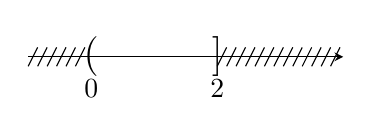
\begin{tikzpicture}[>=stealth, scale=0.8]
					\draw[->] (-1,0) -- (4,0);
					\foreach \x in {-1,-0.85,...,-0.15} \draw (\x,-0.15) -- (\x+0.15,0.15);
					\node at (0,0) {\Large $($};
					\node[below] at (0,-0.2) {$0$};
					\node at (2,0) {\Large $]$};
					\node[below] at (2,-0.2) {$2$};
					\foreach \x in {2,2.15,...,3.85} \draw (\x,-0.15) -- (\x+0.15,0.15);
				\end{tikzpicture}
			\end{center}
			
			\item[b)] Tập hợp các số thực thuộc nửa khoảng $(-4; 2]$ nhưng không thuộc nửa khoảng $[2; 4)$ là khoảng $(-4; 2)$ (vì phần tử $2$ đã bị trừ đi do $2 \in [2; 4)$).\\
			Vậy $(-4; 2] \setminus [2; 4) = (-4; 2)$.\\
			\textbf{Biểu diễn trên trục số:}
			\begin{center}
				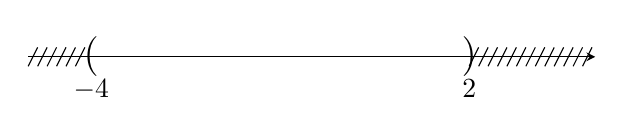
\begin{tikzpicture}[>=stealth, scale=0.8]
					\draw[->] (-5,0) -- (4,0);
					\foreach \x in {-5,-4.85,...,-4.15} \draw (\x,-0.15) -- (\x+0.15,0.15);
					\node at (-4,0) {\Large $($};
					\node[below] at (-4,-0.2) {$-4$};
					\node at (2,0) {\Large $)$};
					\node[below] at (2,-0.2) {$2$};
					\foreach \x in {2,2.15,...,3.85} \draw (\x,-0.15) -- (\x+0.15,0.15);
				\end{tikzpicture}
			\end{center}
			
			\item[c)] $\mathbb{R} \setminus (-1; 1)$ chính là phần bù của $(-1; 1)$ trong $\mathbb{R}$. Tập hợp này gồm các số thực nhỏ hơn hoặc bằng $-1$, và các số thực lớn hơn hoặc bằng $1$.\\
			Vậy $\mathbb{R} \setminus (-1; 1) = (-\infty; -1] \cup [1; +\infty)$.\\
			\textbf{Biểu diễn trên trục số:}
			\begin{center}
				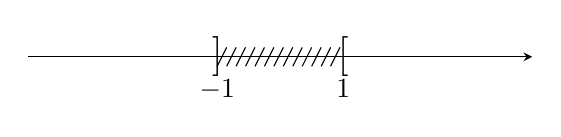
\begin{tikzpicture}[>=stealth, scale=0.8]
					\draw[->] (-4,0) -- (4,0);
					\node at (-1,0) {\Large $]$};
					\node[below] at (-1,-0.2) {$-1$};
					\node at (1,0) {\Large $[$};
					\node[below] at (1,-0.2) {$1$};
					\foreach \x in {-1,-0.85,...,0.85} \draw (\x,-0.15) -- (\x+0.15,0.15);
				\end{tikzpicture}
			\end{center}
		\end{enumerate}
	}
\end{vd}
\dongcham{4}
\begin{vd}
	Cho hai tập hợp $A = \{x \in \mathbb{R} \mid -1 \le x \le 3\}$, $B = \{x \in \mathbb{R} \mid -2 < x < 2\}$. Tìm $A \setminus B, B \setminus A$.
	\loigiai{
		Ta có: $A = [-1; 3]$ và $B = (-2; 2)$.
		\begin{itemize}
			\item $A \setminus B$ là tập các phần tử thuộc $A$ nhưng không thuộc $B$:
			$$ A \setminus B = [-1; 3] \setminus (-2; 2) = [2; 3]. $$
			\item $B \setminus A$ là tập các phần tử thuộc $B$ nhưng không thuộc $A$:
			$$ B \setminus A = (-2; 2) \setminus [-1; 3] = (-2; -1). $$
		\end{itemize}
	}
\end{vd}
\dongcham{4}
\begin{vd}
	Cho hai tập hợp $A = \{x \in \mathbb{R} \mid 1 < x \le 4\}$, $B = \{x \in \mathbb{R} \mid -3 < x\}$. Tìm $C_B A$.
	\loigiai{
		Ta viết lại các tập hợp:
		$A = (1; 4]$ và $B = (-3; +\infty)$.
		Ta thấy mọi phần tử của $A$ đều nằm trong $B$, nên $A \subset B$. 
		Phần bù của $A$ trong $B$ kí hiệu là $C_B A$ và được tính bằng $B \setminus A$:
		$$ C_B A = B \setminus A = (-3; +\infty) \setminus (1; 4] = (-3; 1] \cup (4; +\infty). $$
		Vậy $C_B A = (-3; 1] \cup (4; +\infty)$.
	}
\end{vd}
\dongcham{4}
\begin{vd}
	Cho hai nửa khoảng $A = (-1; 0]$, $B = [0; 1)$. Tìm $A \setminus B$ và $C_{\mathbb{R}} A$.
	\loigiai{
		Ta có:
		\begin{itemize}
			\item $A \setminus B$ là tập hợp các số thuộc $(-1; 0]$ nhưng không thuộc $[0; 1)$. Vì phần tử $0$ nằm trong $B$ nên sẽ bị loại khỏi $A$.
			$$ A \setminus B = (-1; 0] \setminus [0; 1) = (-1; 0). $$
			
			\item $C_{\mathbb{R}} A$ là phần bù của $A$ trong $\mathbb{R}$, tức là $\mathbb{R} \setminus A$.
			$$ C_{\mathbb{R}} A = \mathbb{R} \setminus (-1; 0] = (-\infty; -1] \cup (0; +\infty). $$
		\end{itemize}
	}
\end{vd}
\dongcham{4}
\begin{dang}{Các bài toán biện luận theo tham số}
\end{dang}

\begin{vd}%[0D1B4-1]
	Cho hai tập hợp $A=(-3;5]$, $B=[a;+\infty)$. Tìm $a$ để
	\begin{listEX}[2]%số cột
		\item $A\cap B=[-2;5]$.
		\item $A\cap B$ có đúng một phần tử.
	\end{listEX}
	\loigiai{ \begin{enumerate}
			\item Để $A\cap B=[-2;5]$ khi và chỉ khi $\left\{\begin{aligned}
				&a>-3\\
				&a=-2
			\end{aligned}\right. \Leftrightarrow a=-2$.\\
			Vậy $a=-2$ là giá trị cần tìm.
			\item Để $A\cap B$ có đúng một phần tử khi và chỉ khi $a=5$. Khi đó $A\cap B=\{5\}$.\\
			Vậy $a=5$ là giá trị cần tìm.
		\end{enumerate}
		
	}
\end{vd}\dongcham{6}
\begin{vd}%[0D1K4-1]%
	Cho $A=(-\infty;m+1]$; $B=(-1;+\infty)$. Tìm tất cả giá trị của tham số $m$ để $A \cup B=\mathbb{R}$.
	\loigiai{
		Để $A \cup B=\mathbb{R}$ thì $m+1 \geq -1 \Leftrightarrow m \geq -2$.}
\end{vd}\dongcham{4}


\begin{vd}
	Cho số thực $a<0$ và hai tập hợp $A=\left(-\infty;9a\right)$, $B=\left(\dfrac{4}{a};+\infty \right)$. Tìm $a$ để $A\cap B\ne \varnothing $.
	\loigiai{
		Để hai tập hợp $A$ và $B$ giao nhau khác rỗng khi và chỉ khi $9a>\dfrac{4}{a} \Leftrightarrow 9a^2<4$ (do $a<0$)
		$\Leftrightarrow a^2<\dfrac{4}{9} \Leftrightarrow -\dfrac{2}{3}<a<0$.\\
		Vậy $-\dfrac{2}{3}<a<0$ thỏa mãn yêu cầu bài toán.
	}
\end{vd}\dongcham{4}

\begin{vd}%[0D1B4-1]
	Cho hai tập hợp $A=[-2;m]$, $B=(1;5]$. Tùy theo $m$, xác định tập $B\setminus A$.
	\loigiai{
		Nếu $-2<m\leqslant 1$ thì $A\cap B=\varnothing $. Do đó $B\setminus A=B$.\\
		Nếu $1<m<5$ thì $A\cap B=(1;m)$. Do đó $B\setminus A=B\setminus (1;m)=[m;5]$.\\
		Nếu $m\geqslant 5$ thì $B\subset A$. Do đó $B\setminus A=\varnothing $.
		
	}
\end{vd}\dongcham{8}

\begin{dang}{Ứng dụng thực tế các phép toán tập hợp}
\end{dang}

\begin{vd}%[0D1B3-3]
	Trong kì thi học sinh giỏi cấp trường, lớp 10C1 có $45$ học sinh trong đó có  $17$ bạn đạt học sinh giỏi Văn, $25$ bạn đạt học sinh giỏi Toán và $13$ bạn học sinh không đạt học sinh giỏi. Tìm số học sinh giỏi cả Văn và Toán của lớp 10C1.
	\loigiai{
		\immini{
			\begin{itemize}			
				\item Gọi $A$, $B$ theo thứ tự là tập hợp các học sinh giỏi Văn và giỏi Toán của lớp. 
				Theo đề ta có $|A|=17$, $|B|=25$, $|A\cup B|= 45-13=32$.
				\item Số học sinh giỏi cả Văn và Toán là $$|A \cap B |=|A| + |B| - |A \cup B|=25+17-32=10.$$
			\end{itemize}
		}
		{	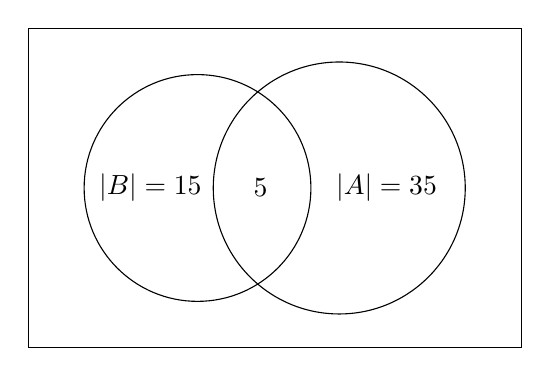
\begin{tikzpicture}[scale=.8]
				\def\radius{2cm}	
				\coordinate (ceni);
				\coordinate[xshift=.9*\radius] (cenii);
				
				\draw (ceni) circle (.9*\radius);
				\draw (cenii) circle (\radius);
				\draw  ([xshift=-25pt,yshift=15pt]current bounding box.north west) 
				rectangle ([xshift=25pt,yshift=-15]current bounding box.south east);
				
				\node[xshift=-.3*\radius] at (ceni) {$|B|=15$};
				\node[xshift=.3*\radius] at (cenii) {$|A|=35$};
				\node[xshift=.4*\radius] at (ceni) {$5$};
	\end{tikzpicture}}}
\end{vd}\dongcham{4}
\begin{vd}%[0D1B3-3]
	Một lớp học có $ 50 $ học sinh trong đó có $ 30 $ em biết chơi bóng chuyền, $25$ em biết chơi bóng đá, $ 10 $ em biết chơi cả bóng đá và bóng chuyền. Hỏi có bao nhiêu em không biết chơi môn nào trong hai môn ở trên?
	\loigiai{
		Gọi tập $A$ là tập hợp các học sinh biết chơi bóng chuyền.
		\\Tập $B$ là tập hợp các học sinh biết chơi bóng đá.
		\\Khi đó số học sinh biết chơi ít nhất một trong hai môn bóng chuyền hoặc bóng đá là 
		$$|A\cup B|=|A|+|B|-|A\cap B|=30+25-10=45.$$
		Vậy số học sinh không biết chơi môn nào là $50-45=5$. 		
	}	
\end{vd}\dongcham{4}

\begin{vd}%[0D1B3-3]
	Lớp $10A$ có $15$ bạn thích môn Văn, $20$ bạn thích môn Toán. Trong số các bạn thích văn hoặc toán có $8$ bạn thích cả $2$ môn. Trong lớp vẫn còn $10$ bạn không thích môn nào trong $2$ môn Văn và Toán. Hỏi lớp $10A$ có bao nhiêu học sinh?
	\loigiai{Ta sử dụng sơ đồ Ven.		
		\begin{center}
			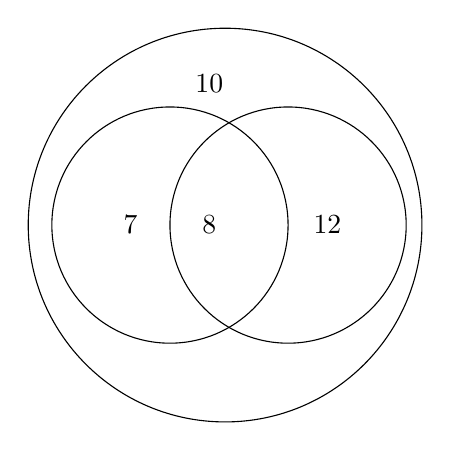
\begin{tikzpicture}
				\draw[] (0.7,0) circle ( 2.5cm);
				\draw[] (0,0) circle ( 1.5cm);
				\draw (1.5,0) circle ( 1.5 cm);
				\draw (-0.5,0) node {$7$};
				\draw (2,0) node {$12$};
				\draw (0.5,0) node {$8$};
				\draw (0.5,1.8) node {$10$};
			\end{tikzpicture}
		\end{center}
		\begin{itemize}
			\item Hình tròn lớn ngoài cùng thể hiện số học sinh cả lớp.\\
			Như vậy, ta có:\\
			\item	Số bạn chỉ thích Văn là $ 15-8=7$(bạn).\\
			\item	Số bạn chỉ thích Toán là $20-8=12$(bạn).\\
			\item	Số học sinh cả lớp là tổng các phần không giao nhau: $7+8+12+10=37$.
		\end{itemize}
	}
\end{vd}\dongcham{4}

\begin{vd}%[0D1K3-3]
	Kết quả thi học kì một của một trường THPT có $48$ thí sinh giỏi môn Toán, $37$ thí sinh giỏi môn Vật Lí, $42$ thí sinh giỏi môn Văn. Biết rằng có $75$ thí sinh giỏi môn Toán hoặc môn Vật lí, $76$ thí sinh giỏi  môn Toán hoặc môn Văn, $66$ thí sinh giỏi môn Vật lí hoặc môn Văn và có $4$ thí sinh giỏi cả ba môn. Hỏi 
	\begin{enumerate}
		\item có bao nhiêu học sinh chỉ giỏi 1 môn.
		\item có bao nhiêu học sinh chỉ giỏi 2 môn.
		\item có bao nhiêu học sinh giỏi ít nhất 1 môn.
	\end{enumerate}
	\loigiai{
		\immini{		
			Gọi $A$, $B$, $C$ theo thứ tự là tập hợp các học sinh giỏi Toán, giỏi Lí và giỏi Văn. Theo đề ta có
			\begin{itemize}
				\item Số học sinh giỏi Toán và Lí là $$|A \cap B=|A|+|B|-|A\cup B|=48+37-75=10.$$	
				\item Số học sinh giỏi Toán và Văn là $$|A \cap C=|A|+|C|-|A\cup C|=48+42 - 76 = 14 .$$	
				\item Số học sinh giỏi Lí và Văn là $$|B \cap C=|B|+|C|-|B\cup C|= 42+37-66=13 .$$	
				\item Số học sinh chỉ giỏi môn Toán $48-10-6-4=28$.	
				\item Số học sinh chỉ giỏi môn Lí $37-6-4-9=18 $.	
				\item Số học sinh chỉ giỏi môn Văn $42-10-9-4=19 $.
			\end{itemize}
		}{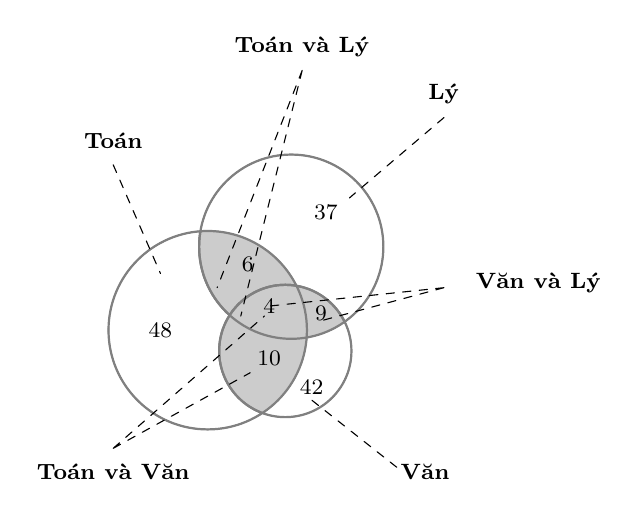
\begin{tikzpicture}[scale=0.6,>=stealth, font=\footnotesize, line join=round, line cap=round]	
				\def\firstcircle{(0,0) circle (2.1cm)}
				\def\secondcircle{(45:2.5cm) circle (1.95cm)}
				\def\thirdcircle{(-15:1.7cm) circle (1.4cm)}
				\colorlet{circle edge}{black!50}
				\colorlet{circle area}{black!20}
				\tikzset{filled/.style={fill=circle area, draw=circle edge, thick},
					outline/.style={draw=circle edge, thick}}
				\draw \firstcircle;
				\draw \secondcircle;
				\draw \thirdcircle;
				\begin{scope}
					\clip \firstcircle;
					\fill[filled] \secondcircle;
				\end{scope}
				\begin{scope}
					\clip \firstcircle;
					\fill[filled] \thirdcircle;
				\end{scope}
				\begin{scope}
					\clip \secondcircle;
					\fill[filled] \thirdcircle;
				\end{scope}  
				\node at (-1,0){48};  
				\node at (2.2,-1.2){42};     
				\node at (2.5,2.5){37}; 
				%
				\node at (0.85,1.4){6}; 
				\node at (1.3,0.5){4}; 
				\node at (1.3,-0.6){10}; 
				\node at (2.4,0.35){9}; 
				\draw[outline] \firstcircle
				\secondcircle  \thirdcircle;    
				\node at (-2,4) {\textbf{Toán}};
				\node at (2,6) {\textbf{Toán và Lý}};
				\node at (5,5) {\textbf{Lý}};
				\node at (7,1) {\textbf{Văn và Lý}};   
				\node at (4.6,-3) {\textbf{Văn}};
				\node at (-2,-3) {\textbf{Toán và Văn}};
				\draw[dashed] (-2,3.5) -- (-1,1.2) 
				(2,5.5) -- (0.7,0.3) 
				(2,5.5) -- (0.2,0.9)
				(5,4.5) -- (3,2.8)
				(5,0.9) -- (1.2,0.5)
				(5,0.9) -- (2.4,0.2)
				(4,-2.9) -- (2.1,-1.4)
				(-2,-2.5) -- (1.2,0.3)
				(-2,-2.5) -- (0.9,-0.9)	;
		\end{tikzpicture}}
		\begin{enumerate}	
			\item Số học sinh chỉ giỏi đúng 1 môn là $28+18+19=65$. 
			\item Số học sinh chỉ giỏi đúng 2 môn là $10+6+9=25$. 
			\item Số học sinh giỏi ít nhất một môn là $65+25+4=94$.
		\end{enumerate}
	}
\end{vd}\dongcham{9}

\boxmini{BÀI TẬP TỔNG HỢP TỰ LUYỆN}

\begin{baitap}
	Cho các tập hợp sau
	\begin{itemize}
		\item [] $A=\left\{\left. x\in \mathbb{Z}\right|-1\le x<6\right\}$;
		\item [] $B=\left\{\left. x\in \mathbb{Q}\right|\left(1-3x\right)\left({x}^4-3x^2+2\right)=0\right\}$;
		\item [] $C=\left\{0;1;2;3;4;5;6\right\}$.
	\end{itemize}
	\begin{tasks}
		\task Viết các tập hợp $A, B$ dưới dạng liệt kê các phần tử.
		\task Tìm $A\cap B,A\cup B,A\backslash B,{C}_{B\cup A}A\cap B$.
		\task Chứng minh rằng $A\cap (B\cup C)=A.$
	\end{tasks}
	\loigiai{
		\begin{enumerate}
			\item Ta có $A=\left\{-1; 0; 1; 2; 3; 4; 5\right\}$, $B=\left\{-1;\dfrac{1}{3};1\right\}$.
			\item Suy ra $A\cap B=\left\{-1;1\right\}$, $A\cup B=\left\{-1;0;\dfrac{1}{3};1;2;3;4;5\right\}$, $A\backslash B=\left\{0;2;3;4;5\right\}$ và ${C}_{B\cup A}\left(A\cap B\right)=\left\{0;\dfrac{1}{3};2;3;4;5\right\}$.
			\item Ta có $B\cup C=\left\{-1;0;1/3;1;2;3;4;5;6\right\}$ suy ra $A\cap \left(B\cup C\right)=\left\{-1;0;1;2;3;4;5\right\}=A$.
		\end{enumerate}
	}
\end{baitap}\cham{10}

\begin{baitap}
	Cho các tập hợp
	\begin{itemize}
		\item [] $A=\left\{\left. x\in \mathbb{R}\right|\left({x}^2+7x+6\right)\left(x^2-4\right)=0\right\}$
		\item [] $B=\left\{\left. x\in \mathbb{N}\right|2x\le 8\right\}$
		\item [] $C=\left\{\left. 2x+1\right|x\in \mathbb{Z}\right.$ và $\left.-2\le x\le 4\right\}$.
	\end{itemize}
	\begin{tasks}
		\task Hãy viết lại các tập hợp $A, B, C$ dưới dạng liệt kê các phần tử.
		\task Tìm $A\cup B$, $A\cap B$, $B\backslash C$, ${C}_{A\cup B}\left(B\backslash C\right)$.
		\task Tìm $\left(A\cup C\right)\backslash B$.
	\end{tasks}
	
	\loigiai{
		\begin{enumerate}
			\item Phương trình $\left({x}^2+7x+6\right)\left(x^2-4\right)=0\Leftrightarrow \hoac{
				& x^2+7x+6=0 \\ 
				& x^2-4=0 \\}\Leftrightarrow \hoac{
				& x=-1\vee x=-6 \\ 
				& x=-2\vee x=2 \\}$.\\
			Vậy $A=\left\{-6;-2;-1;2\right\}$.\\
			Ta có $\heva{
				& x\in \mathbb{N} \\ 
				& 2x\le 8 \\}\Leftrightarrow \heva{
				& x\in \mathbb{N} \\ 
				& x\le 4 \\}\Leftrightarrow x\in \left\{0,1,2,3,4\right\}$. Vậy $B=\left\{0;1;2;3;4\right\}$.\\
			Ta có $\heva{
				& x\in \mathbb{Z} \\ 
				&-2\le x\le 4 \\}\Leftrightarrow x\in \left\{-2,-1,0,1,2,3,4\right\}$. Vậy $C=\left\{-3;-1;1;3;5;7;9\right\}$.
			\item Suy ra $A\cup B=\left\{-6;-2;-1;0;1;2;3;4\right\}$, $A\cap B=\left\{2\right\}$, $B\backslash C=\left\{0;2;4\right\}$, 
			${C}_{A\cup B}\left(B\backslash C\right)=\left(A\cup B\right)\backslash \left(B\backslash C\right)=\left\{-6;-2;-1;1;3\right\}$.
			\item Ta có $A\cup C=\left\{-6;-3;-2;-1;1;2;3;5;7;9\right\}$. Suy ra $(A\cup C)\backslash B=\left\{-6;-3;-2;-1;5;7;9\right\}$.
		\end{enumerate}
	}
\end{baitap}\cham{18}

\begin{baitap}%[Nguyễn Đắc Giáp]%[0D1B4-2]
	Cho đoạn $A=[-5;1]$ và khoảng $B=(-3;2)$. Xác định $A\cup B$, $A\cap B$, $A\setminus B$, $C_{\mathbb{R}}B$.
	\loigiai{
		Ta có
		\begin{itemize}
			\item $A\cup B=[-5;2)$.
			\item $A\cap B=(-3;1]$.
			\item $A\setminus B=[-5;-3]$.
			\item $C_{\mathbb{R}}B=\mathbb{R}\setminus B=(-\infty;-3]\cup [2;+\infty)$.
		\end{itemize} 
	}
\end{baitap}\cham{10}

\begin{baitap}%[Nguyễn Đắc Giáp]%[0D1B4-1]
	Cho các tập hợp $A=\left\{x\in \mathbb{R}\big|x^2\leqslant 4\right\}$, $B=\left\{x\in \mathbb{R}\big|x<1\right\}$. Viết các tập hợp sau đây $A\cup B$, $A\cap B$, $A\setminus B$, $ C_{\mathbb{R}}B$ dưới dạng các khoảng, nửa khoảng, đoạn.
	\loigiai{
		Ta có $A=[-2;2]$ và $B=(-\infty;1)$, suy ra
		\begin{itemize}
			\item $A\cup B=[-2;2]\cup (-\infty;1)=(-\infty;2]$.
			\item $A\cap B=[-2;2]\cap (-\infty;1)=[-2;1)$.
			\item $A\setminus B=[-2;2]\setminus (-\infty;1)=[1;2]$.
			\item $C_{\mathbb{R}}B=[1;+\infty)$.
		\end{itemize}
	}
\end{baitap}\cham{12}

\begin{baitap}%[0D1K4-1]
	Cho các tập hợp $A=\left(-\infty ;m\right)$ và $ B=\left[3m-1;3m+3\right]$. Tìm tất cả những giá trị thực của tham số $ m$ để $ A\cap B=\varnothing $
	\loigiai{
		\immini{Ta có biểu diễn trên trục số các tập $ A$ và $ B$ trên hình vẽ bên\\
			Ta có $ A\cap B=\varnothing $\\
			$\Leftrightarrow m\le 3m-1\Leftrightarrow m\ge\dfrac{1}{2}$\\
			Vậy $ m\ge\dfrac{1}{2}$ là giá trị cần tìm.
		}
		{%
			\begin{tikzpicture}
				\draw[->,>=stealth] (1,0)--(6,0);
				\fill[pattern=north west lines]
				(2,-0.1) rectangle (6,0.1)
				;
				\path
				(2,0) node{)} node[below=2mm] {$ m $}
				;
			\end{tikzpicture}\\%
			\begin{tikzpicture}
				\draw[->,>=stealth] (1,0)--(6,0);
				\fill[pattern=north west lines]
				(1,-0.1) rectangle (2,0.1)
				(4,-0.1) rectangle (6,0.1)
				;
				\path
				(2,0) node{[} node[below=2mm] {$ 3m-1 $}
				(4,0) node{]} node[below=2mm] {$ 3m+3 $}
				;
			\end{tikzpicture}
		}
	}
\end{baitap}\cham{10}

\begin{baitap}%[Trịnh Văn Xuân, latex-k10]%[0D1B4-1]
	Cho các nửa khoảng $A=(a;a+1]$, $B=[b;b+2)$.
	\begin{listEX}[1]
		\item Gọi $C=A\cup B$. Với điều kiện nào của $a, b$ thì $C$ là một đoạn. Tính độ dài của $C$ khi đó.
		\item Gọi $C=A\cap B$. Với điều kiện nào của $a, b$ thì $C$ là một đoạn. Tính độ dài của $C$ khi đó.
	\end{listEX}
	\loigiai{
		Điều kiện: $a, b\in \mathbb{R}$.
		\begin{listEX}[1]
			\item Để $C=A\cup B$ là một đoạn khi và chỉ khi\\
			$b\leqslant a<b+2\leqslant a+1 \Leftrightarrow \left\{\begin{aligned}
				&b\leqslant a<b+2\\
				&b+2\leqslant a+1
			\end{aligned}\right. \Leftrightarrow \left\{\begin{aligned}
				&b\leqslant a<b+2\\
				&b+1\leqslant a
			\end{aligned}\right. \Leftrightarrow b+1\leqslant a<b+2$.\\
			Khi đó $C=[b;b+2)\cup (a;a+1]=[b; a+1]$ là đoạn có độ dài $a-b+1$.
			\item Để $C=A\cap B$ là một đoạn khi và chỉ khi\\
			$a<b<a+1<b+2 \Leftrightarrow \left\{\begin{aligned}
				&a<b\\
				&b<a+1<b+2
			\end{aligned}\right. \Leftrightarrow \left\{\begin{aligned}
				&a<b\\
				&b-1<a<b+1
			\end{aligned}\right. \Leftrightarrow b-1<a<b$.\\
			Khi đó $C=[b;b+2)\cap (a;a+1]=[b; a+1]$ là đoạn có độ dài $a-b+1$.
	\end{listEX}}
\end{baitap}\cham{10}

\begin{baitap}%[Trịnh Văn Xuân, latex-k10]%[0D1B4-1]
	Cho hai tập hợp $A=[a;a+2]$, $B=[b;b+1]$. Tìm điều kiện của $a$, $b$ để $A\cap B\ne \varnothing $.
	\loigiai{
		Ta xét trường hợp $A\cap B=\varnothing $.\\
		Để $A\cap B=\varnothing $ khi và chỉ khi $\left[\begin{aligned}
			&a+2<b\\
			&b+1<a
		\end{aligned}\right. \Leftrightarrow \left[\begin{aligned}
			&a<b-2\\
			&a>b+1
		\end{aligned}\right. $.\\
		Từ đó suy ra điều kiện để $A\cap B\ne \varnothing $ là $b-2\leqslant a\leqslant b+1$.
		
	}
\end{baitap}\cham{12}

\begin{baitap}
	Cho hai tập hợp $A=\left[2;m+1\right]$ và $B=\left[\dfrac{1}{2};+\infty \right)$. Tìm $m$ để $A\cap B$ chỉ có đúng 1 phần tử.
	\loigiai{
		Điều kiện: $2<m+1\Leftrightarrow m>1$.\\
		Để $A\cap B$ chỉ có đúng 1 phần tử khi và chỉ khi $m+1=\dfrac{1}{2}\Leftrightarrow m=-\dfrac{1}{2}$: không thỏa mãn điều kiện.\\
		Vậy không tồn tại giá trị của $m$ để thỏa mãn yêu cầu bài toán.
	}
\end{baitap}\cham{12}


\begin{baitap}%[0D1B3-3]
	Một lớp có $40$ học sinh, mỗi học sinh đều đăng ký chơi ít nhất $1$ trong $2$ môn thể thao là bóng đá hoặc cầu lông. Có $30$ học sinh có đăng ký môn bóng đá, $25$ học sinh có đăng ký môn cầu lông. Hỏi có bao nhiêu em đăng ký cả $2$ môn.
	\loigiai{
		Gọi $A$ là tập hợp các học sinh đăng kí chơi bóng đá, $B$ là tập học sinh đăng kí chơi cầu lông thì $A\cap B$ là tập hợp các học sinh đăng kí chơi cả hai môn.\\	
		Vậy số học sinh đăng kí chơi cả hai môn là 
		$|A\cap B|=|A|+|B|-|A\cup B|=30+25-40=15$. }
\end{baitap}\cham{11}

\begin{baitap}%[0D1B3-3]
	Mỗi học sinh của lớp $10A$ đều chơi bóng đá hoặc bóng chuyền. Biết rằng có $25$ bạn chơi bóng đá, $20$ bạn chơi bóng chuyền và $10$ bạn chơi cả $2$ môn thể thao. Hỏi lớp $10A$ có bao nhiêu học sinh.
	\loigiai{
		Gọi $A$ là tập hợp các học sinh chơi bóng đá, $B$ là tập các học sinh chơi bóng chuyền. Do đó $A\cap B$ là tập các học sinh chơi cả hai môn.\\
		Theo đề $|A|=25$, $|B|=20$, $|A \cap B| =10$.\\
		Vậy số học sinh cả lớp là $|A \cup B| =|A|+|B|-|A\cap B|=25+20-10=35$.}
\end{baitap}\cham{11}

\begin{baitap}%[0D1B3-3]
	Lớp 10A có $45$ học sinh, có $15$ học sinh giỏi và $20$ học sinh xếp hạnh kiểm tốt, trong đó có $10$ bạn vừa học giỏi vừa xếp hạnh kiểm tốt. Các học sinh được học sinh giỏi hoặc hạnh kiểm tốt đều được khen thưởng. Số học sinh được khen thưởng của lớp 10A là là bao nhiêu?
	\loigiai{
		Gọi $A$ là tập hợp các học sinh giỏi, 
		$B$ là tập hợp các học sinh xếp hạnh kiểm tốt.\\
		Khi đó số học sinh được khen thưởng là $|A\cup B|$.\\
		Vậy số học sinh được khen thưởng là 
		$|A\cup B|=|A|+|B|-|A\cap B|=15+20-10=25.$		
	}
\end{baitap}\cham{10}
\begin{baitap}%[0D1K3-3]
	Trong số $42$ học sinh của lớp 10A có $13$ bạn được xếp loại học lực giỏi, $22$ bạn được xếp loại hạnh kiểm tốt, trong đó $7$ bạn vừa học lực giỏi, vừa có hạnh kiểm tốt. Hỏi lớp 10A có bao nhiêu bạn được khen thưởng? Biết rằng muốn được khen thưởng thì bạn đó phải có học lực giỏi hoặc có hạnh kiểm tốt.
	\loigiai{
		Gọi tập hợp các học sinh học lực giỏi là $G$, tập hợp các bạn học sinh hạnh kiểm tốt là $T$. Khi đó tập hợp các bạn học sinh vừa có học lực giỏi là, vừa có hạnh kiểm tốt là $G\cap T$, tập hợp các bạn học sinh đạt học lực giỏi hoặc hạnh kiểm tốt là $G\cup T$. Ta có \\
		$|G|=13$, $|T|=22$, $|G\cap T|=7$.\\
		$|G\cup T|=|G|+|T|-|G\cap T|=13+22-7=28.$}
\end{baitap}\cham{10}

\begin{baitap}%[0D1K3-3]
	Một nhóm học sinh giỏi các bộ môn: Anh, Toán, Văn. Có $ 18 $ em giỏi Văn, $ 10 $ em giỏi Anh, $ 12 $ em giỏi Toán, $ 3 $ em giỏi Văn và Toán, $ 4 $ em giỏi Toán và Anh, $ 5 $ em giỏi Văn và Anh, $ 2 $ em giỏi cả ba môn. Hỏi nhóm đó có bao nhiêu em?
	\loigiai{
		\immini
		{Ký hiệu $ A $ là tập hợp những học sinh giỏi Anh,\\
			$ T $ là tập hợp những học sinh giỏi Toán,\\
			$ V $ là tập hợp những học sinh giỏi Văn.\\
			$\bullet$ $|V|=18,\; |A|=10,\; |T|=12$,\\
			$\bullet$ $|T \cap V|=3,\; |T \cap A|=4,\; |V \cap A|=5, |V \cap A \cap T|=2$.\\
			Số học sinh của nhóm là
			\begin{eqnarray*}
				|V \cup A \cup T|&=&|V|+|A|+|T|-|V \cap A|-|T \cap A|-|T \cap V|\\
				&&+|V \cap A \cap T|\\
				&=&18+10+12-(3+4+5)+2=30.
			\end{eqnarray*}
			Vậy nhóm đó có $ 30 $ em.
		}
		{
			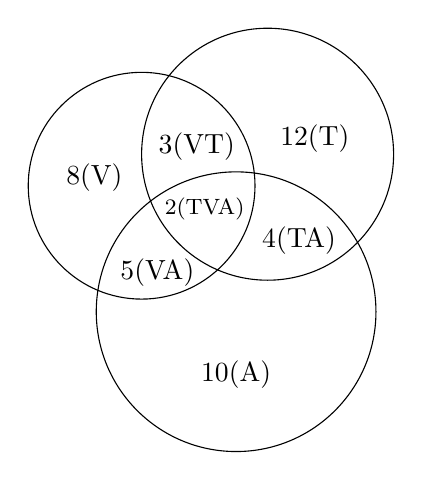
\begin{tikzpicture}[scale=.8]
				\def\radius{2cm}	
				\coordinate (ceni);
				\coordinate[xshift=.8*\radius, yshift=.2*\radius] (cenii);
				\coordinate[xshift=.6*\radius,yshift=-.8*\radius] (ceniii);
				\draw (ceni) circle (.9*\radius);
				\draw (cenii) circle (\radius);
				\draw (ceniii) circle (1.11*\radius);
				
				\node[xshift=-.3*\radius, yshift=.05*\radius] at (ceni) {$8$(V)};
				\node[xshift=.35*\radius, yshift=.25*\radius] at (ceni) {$3$(VT)};
				\node[xshift=.1*\radius, yshift=-.55*\radius] at (ceni) {$5$(VA)};
				\node[xshift=.4*\radius, yshift=-.15*\radius] at (ceni) {{\footnotesize $2$(TVA)}};
				\node[xshift=.2*\radius, yshift=-.55*\radius] at (cenii) {$4$(TA)};
				\node[xshift=1.1*\radius,yshift=.3*\radius] at (ceni) {$12$(T)};
				\node[yshift=-.4*\radius] at (ceniii) {$10$(A)};
			\end{tikzpicture}
		}
	}
\end{baitap}\cham{10}

\begin{baitap}
	Có $44$ học sinh giỏi, mỗi em giỏi ít nhất một môn. Có $22$ em giỏi Văn, $25$ em giỏi Toán, $20$ em giỏi Anh. Có $8$ em giỏi đúng hai môn Văn, Toán; Có $7$ em giỏi đúng hai môn Toán, Anh; Có $6$ em giỏi đúng hai môn Anh, Văn. Hỏi có bao nhiêu em giỏi cả ba môn Văn, Toán, Anh?
	\shortans[oly]{1}
	\loigiai{
		Gọi $V, T, A$ lần lượt là tập hợp các học sinh giỏi môn Văn, Toán, Anh.\\
		Gọi $x$ là số học sinh giỏi cả $3$ môn ($x \in \mathbb{N}$).\\
		Theo giả thiết, số học sinh giỏi đúng $2$ môn là:
		\begin{itemize}
			\item Giỏi đúng Văn và Toán (không giỏi Anh): $8$ em.
			\item Giỏi đúng Toán và Anh (không giỏi Văn): $7$ em.
			\item Giỏi đúng Anh và Văn (không giỏi Toán): $6$ em.
		\end{itemize}
		Từ đó, ta biểu diễn số học sinh chỉ giỏi đúng $1$ môn theo $x$:
		\begin{itemize}
			\item Chỉ giỏi môn Văn: $22 - 8 - 6 - x = 8 - x$.
			\item Chỉ giỏi môn Toán: $25 - 8 - 7 - x = 10 - x$.
			\item Chỉ giỏi môn Anh: $20 - 7 - 6 - x = 7 - x$.
		\end{itemize}
		
		\begin{center}
			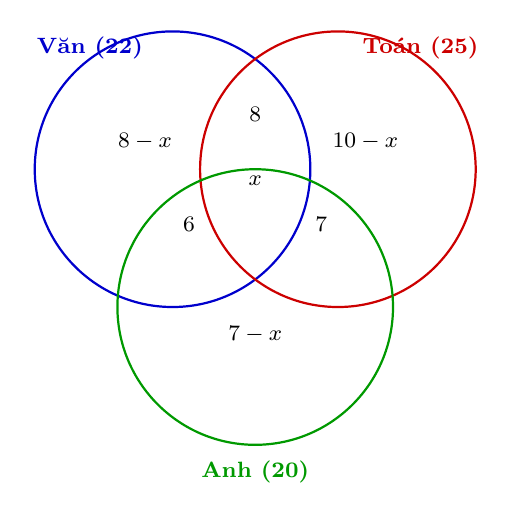
\begin{tikzpicture}[scale=0.7, font=\footnotesize, thick, line join=round, line cap=round]
				% Vẽ các vòng tròn
				\draw[blue!80!black] (0,0) circle (2.5cm);
				\draw[red!80!black] (3,0) circle (2.5cm);
				\draw[green!60!black] (1.5,-2.5) circle (2.5cm);
				
				% Tên các tập hợp
				\node[blue!80!black] at (-1.5, 2.2) {\textbf{Văn (22)}};
				\node[red!80!black] at (4.5, 2.2) {\textbf{Toán (25)}};
				\node[green!60!black] at (1.5, -5.5) {\textbf{Anh (20)}};
				
				% Các giá trị trong biểu đồ
				\node at (-0.5, 0.5) {$8-x$};
				\node at (3.5, 0.5) {$10-x$};
				\node at (1.5, -3) {$7-x$};
				
				\node at (1.5, 1) {$8$};
				\node at (0.3, -1) {$6$};
				\node at (2.7, -1) {$7$};
				
				\node at (1.5, -0.2) {$x$};
			\end{tikzpicture}
		\end{center}
		
		Vì tổng số học sinh là $44$ và mỗi em đều giỏi ít nhất một môn nên tổng các phần trong biểu đồ Venn phải bằng $44$. Ta có phương trình:
		$$ (8 - x) + (10 - x) + (7 - x) + 8 + 7 + 6 + x = 44 $$
		$$ \Leftrightarrow 46 - 2x = 44 \Leftrightarrow 2x = 2 \Leftrightarrow x = 1. $$
		Vậy có đúng $1$ em học sinh giỏi cả ba môn Văn, Toán, Anh.
	}
\end{baitap}
